% Compile with XeLaTeX, TeXLive 2013 or more recent
\documentclass{beamer}

% Base packages
\usepackage{fontspec}
\usepackage{xunicode}
\usepackage{xltxtra}

\usepackage{amsfonts}
\usepackage{amsmath}
\usepackage{longtable}
\usepackage{csquotes}
\usepackage{standalone}

% Setup fonts
\newfontfamily\russianfont{CMU Serif}
\setromanfont{CMU Serif}
\setsansfont{CMU Sans Serif}
\setmonofont{CMU Typewriter Text}

% Setup Russian hyphenation. NOTE: this declaration *must* come after fontspec's font declarations,
% or a mysterious (but harmless in other respects) error "Improper `at' size (0.0pt), replaced by 10pt." would appear.
\usepackage{polyglossia}
\defaultfontfeatures{Scale=MatchLowercase, Mapping=tex-text}

\setdefaultlanguage[spelling=modern]{russian} % for polyglossia
\setotherlanguage{english} % for polyglossia

% Vector drawings 
\usepackage{tikz}
\usetikzlibrary{shapes, calc, arrows, fit, positioning, decorations, patterns, decorations.pathreplacing, chains, snakes}
\usepackage[siunitx]{circuitikz}

% Be able to insert hyperlinks
\usepackage{hyperref}
\hypersetup{colorlinks=true, linkcolor=black, filecolor=black, citecolor=black, urlcolor=blue , pdfauthor=Grigory Rechistov <grigory.rechistov@phystech.edu>, pdftitle=Моделирование OpenRISC 1000 на Wind River Simics}
% \usepackage{url}

% Misc optional packages
\usepackage{underscore}
\usepackage{amsthm}

% A new command to mark not done places
\newcommand{\todo}[1][Напиши меня]{{\color{red}TODO\ #1}}

\title{Создание программных моделей устройств}
% \subtitle{Курс «Программное моделирование вычислительных систем»}
\subject{Лекция}
\author[Григорий Речистов]{Григорий Речистов \\ \small{\href{mailto:grigory.rechistov@intel.com}{grigory.rechistov@intel.com}}}
\date{26-28 августа 2014 г.}
\pgfdeclareimage[height=0.5cm]{intel-logo}{../images/intel.png}
\logo{\pgfuseimage{intel-logo}}


\usetheme{Berlin}
\setbeamertemplate{navigation symbols}{}%remove navigation symbols

\begin{document}

\begin{frame}
\titlepage
\end{frame}

\begin{frame}
\tableofcontents
\end{frame} 

\section{Что моделируем}
\centering
\begin{frame}{Схема платформы}

\begin{tikzpicture}[>=stealth, font=\small, node distance = 0.4cm]


\begin{scope}[minimum height=0.8cm]
	\node[draw, ] (cpu) {CPU};
	\node[draw, below=of cpu] (mmu) {MMU};
	\node[draw, right=3cm of cpu, ] (pic) {PIC};
	\node[draw, left=of cpu, ] (caches) {L\$};

	\node[draw, below=of mmu, text width=3cm, align = center, ] (dram) {DRAM};
	\node[draw, left=of dram, ] (pmu) {PMU};
	\node[draw, right=of dram, ] (rom) {ROM};
	\node[draw, right=of rom, ] (dev-A) {\footnotesize Bridge A};

	\node[draw, right=of dev-A, ] (dev-B) {\footnotesize Bridge B};
	\node[draw, right=of dev-B, ] (pit) {PIT};

	\node[draw, below=of dev-A, ] (video) {Video};
	\node[draw, below=of video, ] (monitor) {Monitor};

	\node[draw, below=of dev-B, ] (usb-1) {\tiny USB Dev 1};
	\node[draw, below=of dev-B, xshift=1.5cm] (usb-2) {\tiny USB Dev 2};
\end{scope}

\draw[<->] (cpu) -- (mmu);
\draw[<->] (cpu) -- (caches);
\draw[<->] (mmu) -- (dram);

\draw[<->] (mmu) -| (rom);
\draw[<->] (mmu) -| (pmu);
\draw[<->] (mmu) -| (dev-A);
\draw[<->] (mmu) -| (dev-B);
\draw[<->] (mmu) -| (pit);

\draw[->, dashed] (pic) -- (cpu);
\draw[->, dashed] (pit) -- (pic);
\draw[->, dashed] (dev-A) -- (pic);
\draw[->, dashed] (dev-B) -- (pic);

\draw[<->] (dev-A) -- (video);
\draw[<->] (video) -- (monitor);

\draw[<->] (dev-B) -- (usb-1);
\draw[<->] (dev-B) -- (usb-2);

\path[->, draw, dotted] (pmu.west) -- ([xshift=-0.3cm]pmu.west) |- ([yshift=0.3cm]cpu.north) -- (cpu.north);
\path[->, draw, dotted] (pmu.south) -- ([yshift=-0.25cm]pmu.south) -| (dram.235);
\path[->, draw, dotted] (pmu.south) -- ([yshift=-0.25cm]pmu.south) -| (dev-A.235);
\path[->, draw, dotted] (pmu.south) -- ([yshift=-0.25cm]pmu.south) -| (dev-B.235);


\end{tikzpicture}

\end{frame} 

\section{Типы моделей}

\begin{frame}{Типы моделей}

\begin{itemize}
\item Исполняющие (execution-driven)
\item Неисполняющие (event-driven)

\end{itemize}


% \begin{tikzpicture}[>=latex, font=\small]

% \begin{scope}[minimum width = 8cm, node distance = 0.2cm, inner sep=2pt]

% \node[draw, ] (schematics) {Схемотехника};
% \node[draw, above = of schematics] (digital) {Цифровая электроника};
% \node[draw, above = of digital] (rtl-design) {Проектирование микросхем};
% \node[draw, above = of rtl-design] (transactions) {Разработка стандартов передачи данных};
% \node[draw, thick, above = of transactions] (simulation) {\bfseries Симуляция};
% \node[draw, above = of simulation] (firmware) {Firmware};
% \node[draw, above = of firmware] (oses) {Операционные системы};
% \node[draw, above = of oses] (drivers) {Драйверы};
% \node[draw, above = of drivers] (compilers) {Компиляторы};
% \node[draw, above = of compilers] (software) {Прикладные программы};
% \node[draw, above = of software] (algorithms) {Алгоритмы};

% \end{scope}
% \end{tikzpicture}

\end{frame}

\section{Интерпретация}

\begin{frame}{Конвеер центрального процессора}

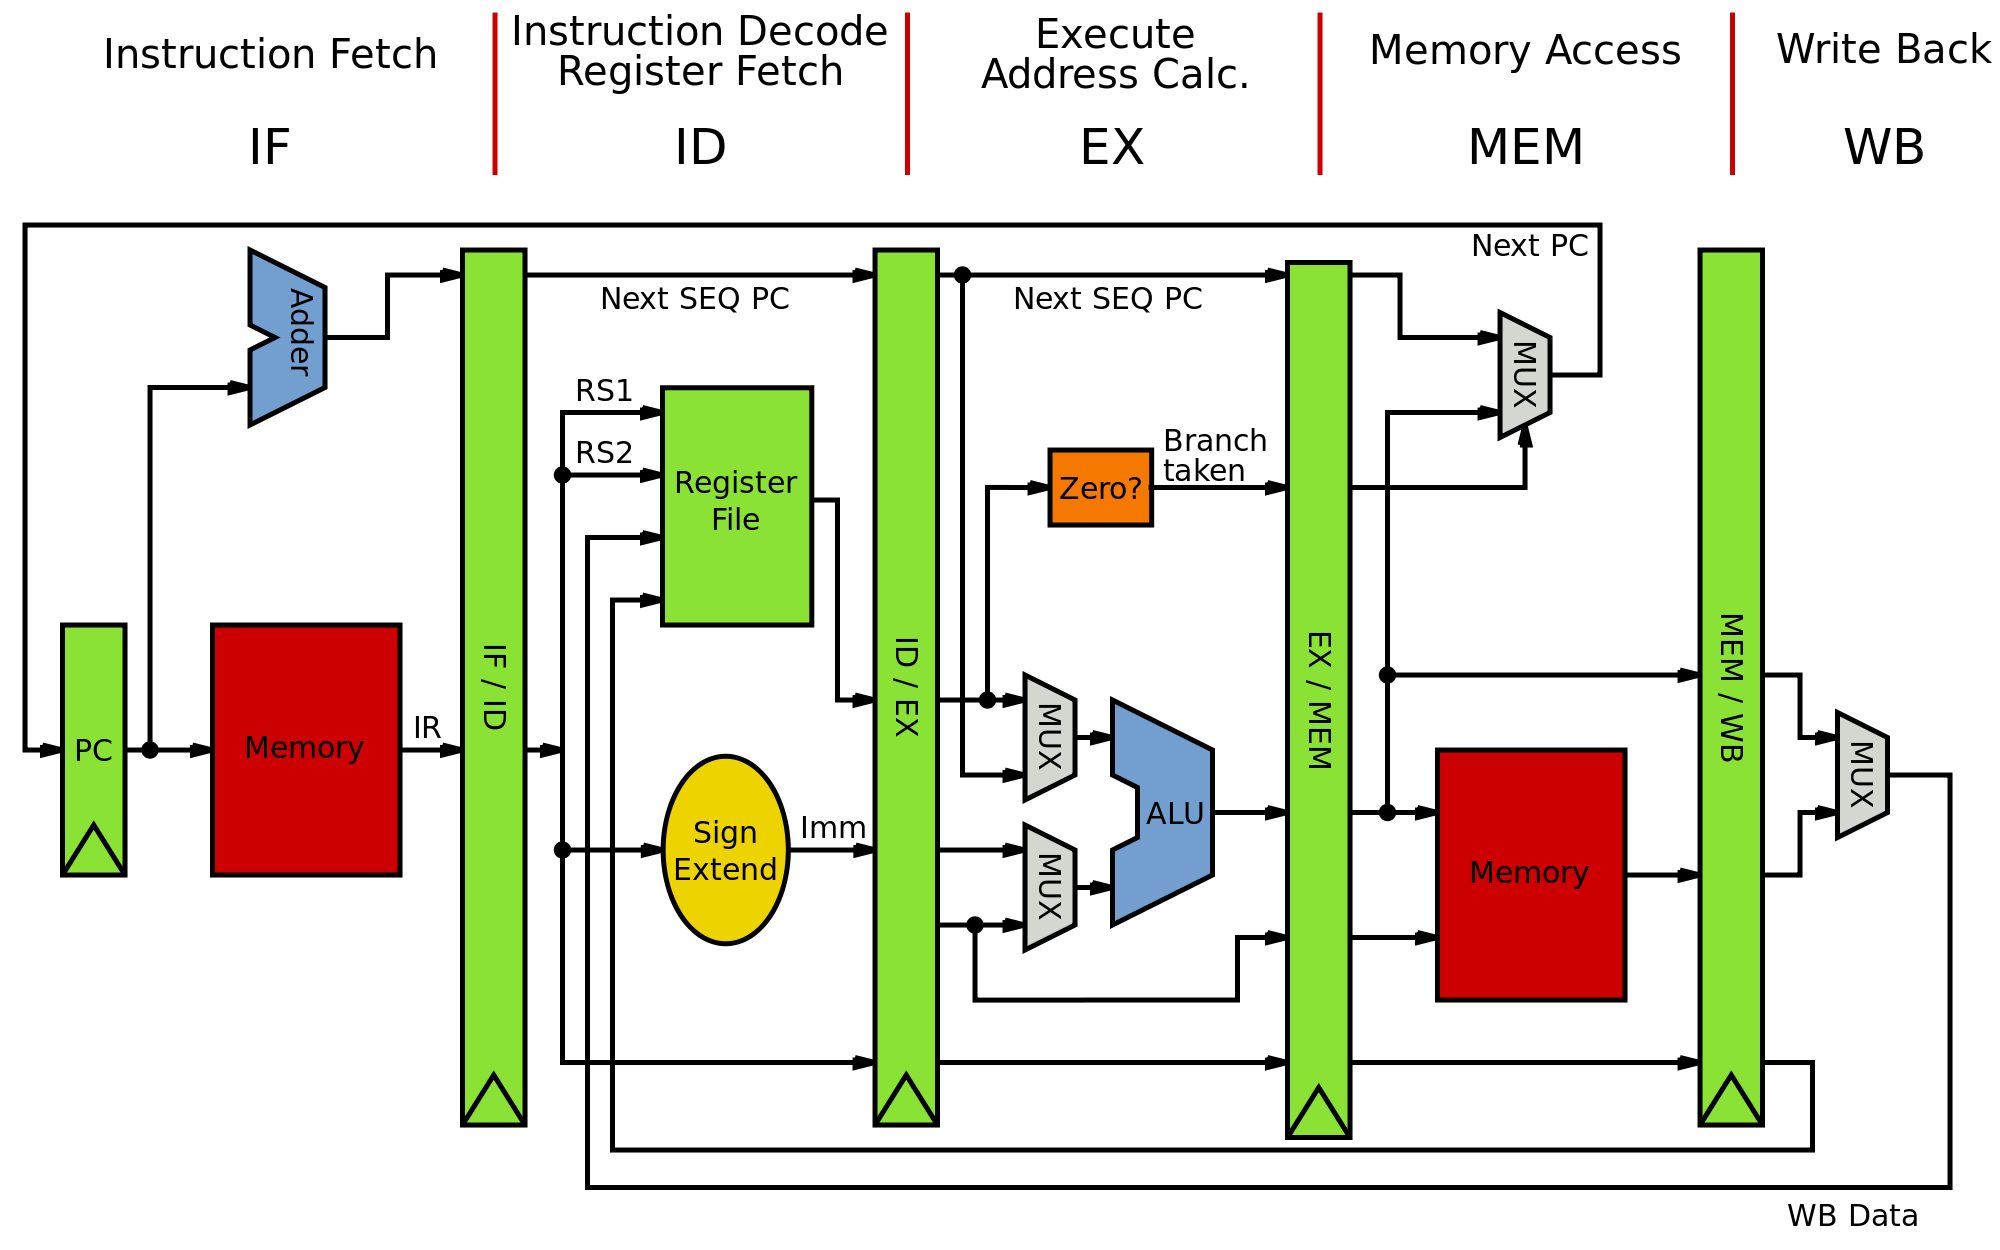
\includegraphics[width=0.8\textwidth]{mips-pipeline}

\tiny{Источник: \url{http://commons.wikimedia.org/wiki/File:MIPS_Architecture_(Pipelined).svg}}

\end{frame} 


\begin{frame}{Цикл симуляции одной инструкции}

\centering

\begin{tikzpicture}[font=\footnotesize, >=latex]
	% five circles
	\foreach \A/\T in    { 90/{Извлечь инструкцию},
						   18/{Декодировать},
						  306/{Исполнить},
						  234/{Запись в память},
						  162/{Продвинуть \texttt{PC}}
		} {
		\node[draw, circle, text width = 2cm, text badly centered](stage\A) at (\A:2.5cm) {\small\T};
		}
		% arrows, dumb way
		\draw[->, ] (stage90) -- (stage18);
		\draw[->, ] (stage18) -- (stage306);
		\draw[->, ] (stage306) -- (stage234);
		\draw[->, ] (stage234) -- (stage162);
		\draw[->, ] (stage162) -- (stage90);
\end{tikzpicture}

\end{frame} 


\begin{frame}[fragile]{Интерпретация}

\begin{verbatim}
while (true) {
	raw_instr = fetch(PC);
	(opcode, operands)= decode(raw_instr);
	switch (opcode) {
		case ADD: do_add(operands);
		case MUL: do_mul(operands);
		case MOV: do_mov(operands);
		...
		default: UD_fault();
	}
	PC += INSTR_SIZE;
}
\end{verbatim}

\end{frame} 

\section{DES}

\begin{frame}{Дискретное моделирование событий}

\centering
\begin{tikzpicture}[>=latex, font=\scriptsize]
    \draw[->] (0,0) -- (10,0) node[pos=0.9, below] (sim-time) {Время};

    \foreach \x in { 1, 2, 3, 4, 5, 6, 7, 8, 9} { 
        \draw (\x,-0.15) -- (\x,0.15) node (tick\x) {};
    };
    \node[shape=dart, draw, shape border rotate=270 ] at (2, 0.5) (currevent) {};
    \node[draw, arrow box, arrow box arrows={north:.7cm}, text width=2.5cm, align=center, below = 0cm of currevent] (tsim) {Текущее симулируемое время};
    \node[align=center, above=0.2cm of currevent, text width=2cm]  {Обрабатываемое событие};
    
    \node[shape=dart, draw, shape border rotate=270 ] at (5, 0.5) (futureevent) {};
    \node[align=center, above=0.2cm of futureevent, text width=2cm] {Запланированное событие};
    
    \node[fill=black!10, shape=dart, draw, shape border rotate=270 ] at (7, 0.5) (newbornevent) {};
    \node[align=center, above=0.2cm of newbornevent, text width=1.5cm] {Новое событие};
    
    \node[shape=dart, draw, shape border rotate=270 ] at (9, 0.5) (futureevent2) {};
    \node[shape=dart, draw, shape border rotate=270, above=0cm of futureevent2 ] (futureevent3) {};
    
    \draw[dashed, ->] (currevent.south) .. controls +(1,-0.5) and +(-1,-0.5) .. (newbornevent.south); % node[below, pos=0.7, text width=3cm] {Обработка события порождает новое событие в будущем};
        
\end{tikzpicture}

\end{frame} 


\begin{frame}{Совместная работа двух классов моделей}

\begin{tikzpicture}[>=latex]
    \node[draw, circle, text width = 3cm, text badly centered] (dessim) {Симулятор дискретных событий};
    \node[draw, circle, text width = 3cm, text badly centered, right = 2.5cm of dessim] (execsim) {Модель исполняющего устройства};
    
    \draw (dessim.45)   edge[bend left = 45, ->] (execsim.135);
    \node[above=1cm of execsim.135] {\small Длительность до следующего события};
    \draw (execsim.225) edge[->, bend left = 45] (dessim.315);
    \node[below=1cm of dessim.315] {\small Число исполненных шагов};
    
\end{tikzpicture}


\end{frame} 



% \section{Литература}

% \begin{frame}[allowframebreaks]{Литература}
% \begin{thebibliography}{99}
    % \bibitem{simbook} Программное моделирование вычислительных систем (лекции) \url{http://atakua.doesntexist.org/public/archive/simcourse/simulation-lectures-latest.pdf}
	
	% \bibitem{practicum} Лабораторный практикум по программному моделированию.  \url{http://atakua.doesntexist.org/public/archive/simcourse/simulation-practicum-latest.pdf}

% \end{thebibliography}
% \end{frame}


\section{Конец}
% The final "thank you" frame 
\begin{frame}

{\huge{Спасибо за внимание!}\par}

\vfill

Слайды и материалы курса доступны по адресу \url{http://bit.ly/1y1lZF1} % http://atakua.doesntexist.org/wordpress/tag/or1k/

\vfill

\tiny{\textit{Замечание}: все торговые марки и логотипы, использованные в данном материале, являются собственностью их владельцев. Представленная точка зрения отражает личное мнение автора.
%Материалы доступны по лицензии Creative Commons Attribution-ShareAlike (Атрибуция — С сохранением условий) 4.0 весь мир (в т.ч. Россия и др.). Чтобы ознакомиться с экземпляром этой лицензии, посетите \url{http://creativecommons.org/licenses/by-sa/4.0/}
}

\end{frame}

% \section{Резерв}

\end{document}


